% ============================================================
%  Chapter 2 — Related Work
% ============================================================
\chapter{Related Work}
\label{ch:related}

The purpose of this chapter is to place CIAI among prior work: what earlier IID methods
assume about the illuminant, how training on one scene under several lights has been used
before, and which benchmarks can test stability and accuracy.
We cover classical and learning-based IID methods in Sections \ref{sec:classical_iid}
and \ref{sec:learning_iid}, work on multi-illuminant scenes and colour constancy in
\secref{sec:multiillum}, and the evaluation benchmarks we use in \secref{sec:benchmarks}.


\section{Classical Intrinsic Image Decomposition}
\label{sec:classical_iid}

The problem of separating illumination from reflectance is rooted in Retinex
theory \mycite{land71retinex}. Its starting observation is that perceived
lightness depends strongly on spatial comparisons, not only on the number
recorded at one pixel. If neighbouring image intensities are $I_1=A_1S_1$ and
$I_2=A_2S_2$, their ratio is
\begin{equation}
  \frac{I_1}{I_2}=\frac{A_1}{A_2}\frac{S_1}{S_2}.
  \label{eq:retinex_ratio}
\end{equation}
When illumination varies slowly over that small neighbourhood,
$S_1/S_2\approx1$, so the observed ratio is evidence for a reflectance change.
For example, a painted black stripe on a white wall should remain a material
boundary as the room becomes brighter. A soft illumination gradient should not.
Retinex-style methods classify or threshold such local changes and propagate the
surviving ratios to estimate a reflectance field.

This is foundational because it turns an impossible per-pixel factorisation into
a problem that can use spatial context. It is also only a prior. A hard cast
shadow can change abruptly and resemble paint; textured material can vary rapidly;
specular highlights violate the diffuse product model. The common shorthand
``illumination is low-frequency and reflectance is high-frequency'' is therefore
a useful intuition, not a physical rule. Modern learned methods replace many
hand-designed thresholds with data, but they still rely on the same distinction
between material changes and lighting changes.

\figref{fig:retinex_ambiguity} shows why such assumptions are necessary. Even a
simple brightness gradient has multiple exact decompositions: the image alone
does not reveal whether the change came from the surface or the light.
\begin{figure}[t!]
  \centering
  \resizebox{\textwidth}{!}{%
  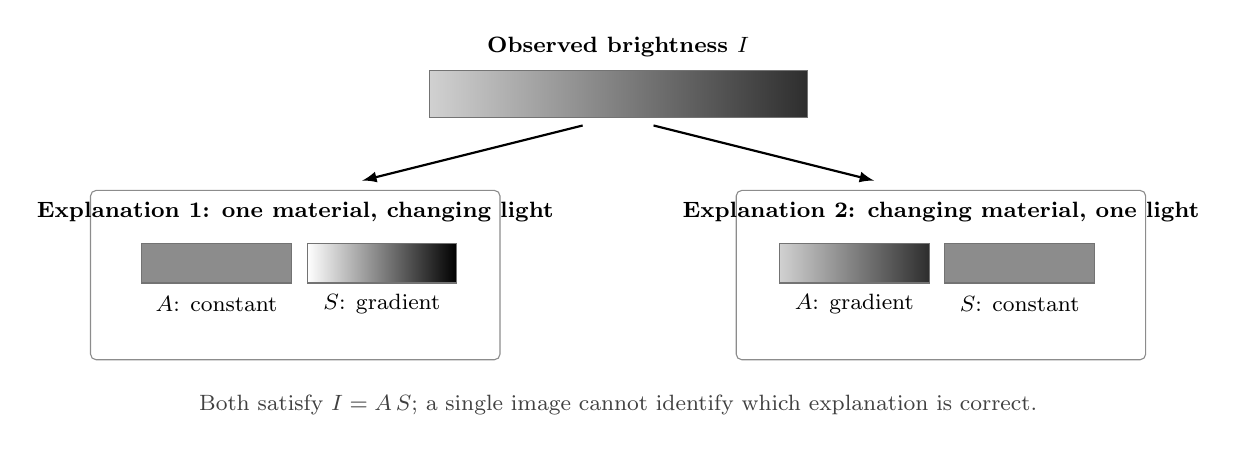
\begin{tikzpicture}[
    font=\small,
    >=latex,
    box/.style={draw=black!45, rounded corners=2pt, inner sep=7pt},
    lab/.style={font=\footnotesize\bfseries, align=center}
  ]
    \node[lab] at (0,1.55) {Observed brightness $I$};
    \shade[left color=black!18,right color=black!82,draw=black!55]
      (-2.4,0.65) rectangle (2.4,1.25);

    \node[box, minimum width=5.2cm, minimum height=2.15cm] at (-4.1,-1.35) {};
    \node[lab] at (-4.1,-0.55) {Explanation 1: one material, changing light};
    \fill[black!45,draw=black!55] (-6.05,-1.45) rectangle (-4.15,-0.95);
    \shade[left color=white,right color=black,draw=black!55]
      (-3.95,-1.45) rectangle (-2.05,-0.95);
    \node[font=\footnotesize] at (-5.1,-1.72) {$A$: constant};
    \node[font=\footnotesize] at (-3.0,-1.72) {$S$: gradient};

    \node[box, minimum width=5.2cm, minimum height=2.15cm] at (4.1,-1.35) {};
    \node[lab] at (4.1,-0.55) {Explanation 2: changing material, one light};
    \shade[left color=black!18,right color=black!82,draw=black!55]
      (2.05,-1.45) rectangle (3.95,-0.95);
    \fill[black!45,draw=black!55] (4.15,-1.45) rectangle (6.05,-0.95);
    \node[font=\footnotesize] at (3.0,-1.72) {$A$: gradient};
    \node[font=\footnotesize] at (5.1,-1.72) {$S$: constant};

    \draw[->,thick] (-0.45,0.55) -- (-3.25,-0.15);
    \draw[->,thick] (0.45,0.55) -- (3.25,-0.15);
    \node[font=\footnotesize,align=center,text=black!75] at (0,-3.0)
      {Both satisfy $I=A\,S$; a single image cannot identify which explanation is correct.};
  \end{tikzpicture}
  }
  \caption[Why intrinsic decomposition is ambiguous.]{%
    The intrinsic-image ambiguity in one dimension. The same observed brightness
    gradient can be explained by constant reflectance under changing illumination
    (left), or by changing reflectance under constant illumination (right).
    Retinex and learned IID methods resolve this underdetermined factorisation by
    adding spatial, semantic, and data-derived priors.
  }
  \label{fig:retinex_ambiguity}
\end{figure}


\mycitetext{grosse09mit} introduced the MIT Intrinsic Images dataset,
the first public benchmark for IID, and used it to show that simple Retinex
baselines outperformed more sophisticated methods of the time on real photographs.
A consistent finding from this benchmark is that the problem is extremely
ill-posed: many different (albedo, shading) pairs explain the same image.
Without strong priors, models tend to find trivial solutions.

The most influential approach to adding structure to the ill-posed problem is
Shape, Illumination, and Reflectance from Shading (SIRFS) by
\mycitetext{barron15sirfs}.
SIRFS frames IID as an energy minimisation over albedo, shading, and surface
normals jointly.
It encodes strong priors: albedos should be piecewise-constant, shadings should be
smooth, and surface normals should form a plausible scene geometry.
SIRFS significantly outperformed previous methods and remained a strong baseline
for several years.
However, its hand-designed priors struggle on complex real-world scenes with
cluttered backgrounds, unusual lighting, or materials that violate the
piecewise-constant albedo assumption.


\section{Learning-Based Intrinsic Image Decomposition}
\label{sec:learning_iid}

The availability of large synthetic datasets shifted the field toward learned models.
\mycitetext{li18cgintrinsics} proposed CGIntrinsics, a set of physically-based
re-renderings of synthetic indoor scenes that provides paired
(image, albedo, shading) training data at scale.
They showed that a CNN trained on this data, combined with ordinal supervision
from the human judgements of IIW \mycite{bell14iiw}, generalises well to real
photographs.
CGIntrinsics established the pattern that has dominated the field since:
train on photorealistic synthetic data with ground-truth labels, then evaluate
on real images.

\mycitetext{bell14iiw} introduced the Intrinsic Images in the Wild (IIW) benchmark of human
lightness judgements (\secref{sec:benchmarks}), which became the field's standard test of
real photographs, although it measures relative lightness rather than material colour.

A line of work by Careaga and Aksoy is the closest to ours in its treatment of
illumination colour.
Ordinal Shading \mycite{careaga23ordinal} decomposes real photographs by first
estimating shading up to an ordinal (ordering) constraint, which is far more
robust than absolute regression, and then refining the albedo; its shading is
still greyscale.
Its successor, Colorful Diffuse IID (CD-IID) \mycite{careaga24cdiid}, is the
first method to explicitly predict a \emph{coloured} diffuse shading in the wild,
through a multi-stage cascade (grey decomposition, then a low-resolution
chromaticity network, then albedo and diffuse-shading refinement) and an analytic
non-diffuse residual.
CD-IID is the direct point of comparison for this work. It trains each stage on single
images, including MIDIntrinsics, and uses no loss that ties the albedos of two
illuminations of one scene together. Its colour separation instead comes from the
architecture: a dedicated stage that predicts the chromaticity of the shading. Our
measurements in \chapref{ch:experiments} suggest that this structural choice, rather than
any amount of paired supervision on MID, is what makes its albedo colour-stable, and the
model we plan next adopts the same split.

In parallel, diffusion-based models have become strong IID baselines.
Marigold-IID \mycite{marigoldiid24} fine-tunes a Stable-Diffusion backbone for
IID and ships two variants: an \emph{appearance} model trained on InteriorVerse
that targets material properties (albedo, roughness, metallic), and a
\emph{lighting} model trained on Hypersim \mycite{roberts21hypersim} that targets
albedo, diffuse shading, and a non-diffuse residual.
Both produce visually sharp decompositions and excellent zero-shot WHDR on IIW.
We use Marigold-IID as our primary experimental baseline because checkpoints are
public, its lighting variant shares our model's training distribution (Hypersim), and
it represents the current generative state of the art.
Very recent work reaches for external knowledge instead: ReasonX
\mycite{reasonx25} guides the decomposition with a multimodal language model and
reports strong IIW WHDR improvements; no public checkpoint was available at the
time of writing, so we cite its published numbers only where protocols match.

Of these, Marigold-IID, CRefNet, Ordinal Shading, CD-IID and RGB$\rightarrow$X
\mycite{zeng24rgbx} are run locally in \chapref{ch:experiments}; the others are cited from
their papers (\secref{sec:exp_setup}).

What these methods share is that each image is decomposed, and supervised, on its own.
Nothing in a single-image objective tells the model that two photographs of the same
room should yield the same albedo, so whatever lighting the priors fail to explain, in
brightness or in colour, can remain in the albedo and differ from one photograph to the
next. Our work adds that cross-image constraint during training, using real
multi-illumination photographs, and measures what it fixes and what it does not.


\section{Multi-Illuminant Scenes and Colour Constancy}
\label{sec:multiillum}

The specific challenge of coloured illumination in IID has received relatively
little attention compared to the broader IID problem.
Most methods implicitly assume a single white or near-white illuminant.

With a scalar shading, a coloured illuminant can only go into the albedo
(\secref{sec:physics}); this section covers how prior work has responded.

\paragraph{Training on one scene under several illuminations}
Using several images of a static scene under changing light is an old idea in IID:
the reflectance is shared across the images while the illumination is not.
\mycitetext{li18bigtime} learn a single-image decomposition from time-lapse sequences
with losses that require a common reflectance across frames.
\mycitetext{lettry18unsupervised} train a Siamese network on illumination-varying
sequences, requiring the reflectances of two frames to agree and their cross-combined
factors to reconstruct the images.
\mycitetext{ma18single} train a two-stream network without ground-truth intrinsic images on
pairs of the same scene under different illumination, and reduce it to a single stream at
inference. These works use the paired constraint as the \emph{main} supervision, mostly on
time-lapse or synthetic sequences. We use it instead as a second training stage on top of
supervised synthetic training, on real raw multi-illumination photographs, and measure
separately what it does to luminance and to colour. The constraint is also close in spirit
to Siamese representation learning without negatives \mycite{chen21simsiam}, where two
views of one object must map to one representation.

\tabref{tab:paired_work} summarises how these works, and the two methods closest to ours,
use images of one scene under several lights.

\begin{table}[t!]
  \caption[Training on one scene under several lights.]{%
    How prior work uses images of one scene under several lights, compared with CIAI. All
    methods take a single image at inference.
  }
  \label{tab:paired_work}
  \centering
  \small
  \begin{tabularx}{\textwidth}{@{}>{\raggedright\arraybackslash}p{0.27\textwidth}>{\raggedright\arraybackslash}X>{\raggedright\arraybackslash}X@{}}
    \toprule
    Method & Where the pairs come from & How the pairs are used \\
    \midrule
    \mycitetext{li18bigtime} & Real time-lapse sequences & Main supervision (shared reflectance) \\
    \mycitetext{lettry18unsupervised} & Illumination-varying sequences & Main supervision (Siamese) \\
    \mycitetext{ma18single} & Pairs of one scene under two lights & Main supervision (two streams) \\
    \mycitetext{kinoshita21consistency} & Simulated illumination variants & Main supervision (reflectance consistency) \\
    CD-IID \mycite{careaga24cdiid} & None & Single images; colour from a shading-chroma stage \\
    \midrule
    CIAI (ours) & Real raw MID flash pairs & Second stage after supervised synthetic training \\
    \bottomrule
  \end{tabularx}
\end{table}

The closest prior work in its treatment of illuminant colour is the self-supervised
decomposition network of \mycitetext{kinoshita21consistency}.
They observe the same gap we do: most IID methods do not enforce any consistency
on the \emph{reflectance} layer, and the usual white-illuminant model cannot
express a coloured light in the first place.
Their answer is to adopt a colour-illuminant model and to train with losses
computed over several illumination conditions of the same content, so that the
predicted reflectance is pushed to agree across them.
The difference from our work lies in where those conditions come from.
Their illumination variants are \emph{simulated}, which makes the supervision
cheap but ties it to the realism of the simulator.
We instead take the constraint from real photographs of real rooms
(\secref{sec:mid_dataset}). The cost of that choice, measured in
\chapref{ch:experiments}, is that the real corpus available varies the direction and
intensity of a white light far more than its colour.


\section{Evaluation Benchmarks}
\label{sec:benchmarks}

We evaluate our model on four benchmarks that together cover different aspects of IID
quality.

The four benchmarks answer different questions. MID tests whether a real
surface stays stable across lights; MAW measures real material colour on sampled
regions; ARAP provides dense synthetic albedo and repeated illumination; IIW
tests whether predicted relative reflectance agrees with people. No single score
is treated as a complete definition of IID quality.
\figref{fig:datasets} shows one example of each benchmark and the ground truth it provides.

\begin{figure}[t!]
  \centering
  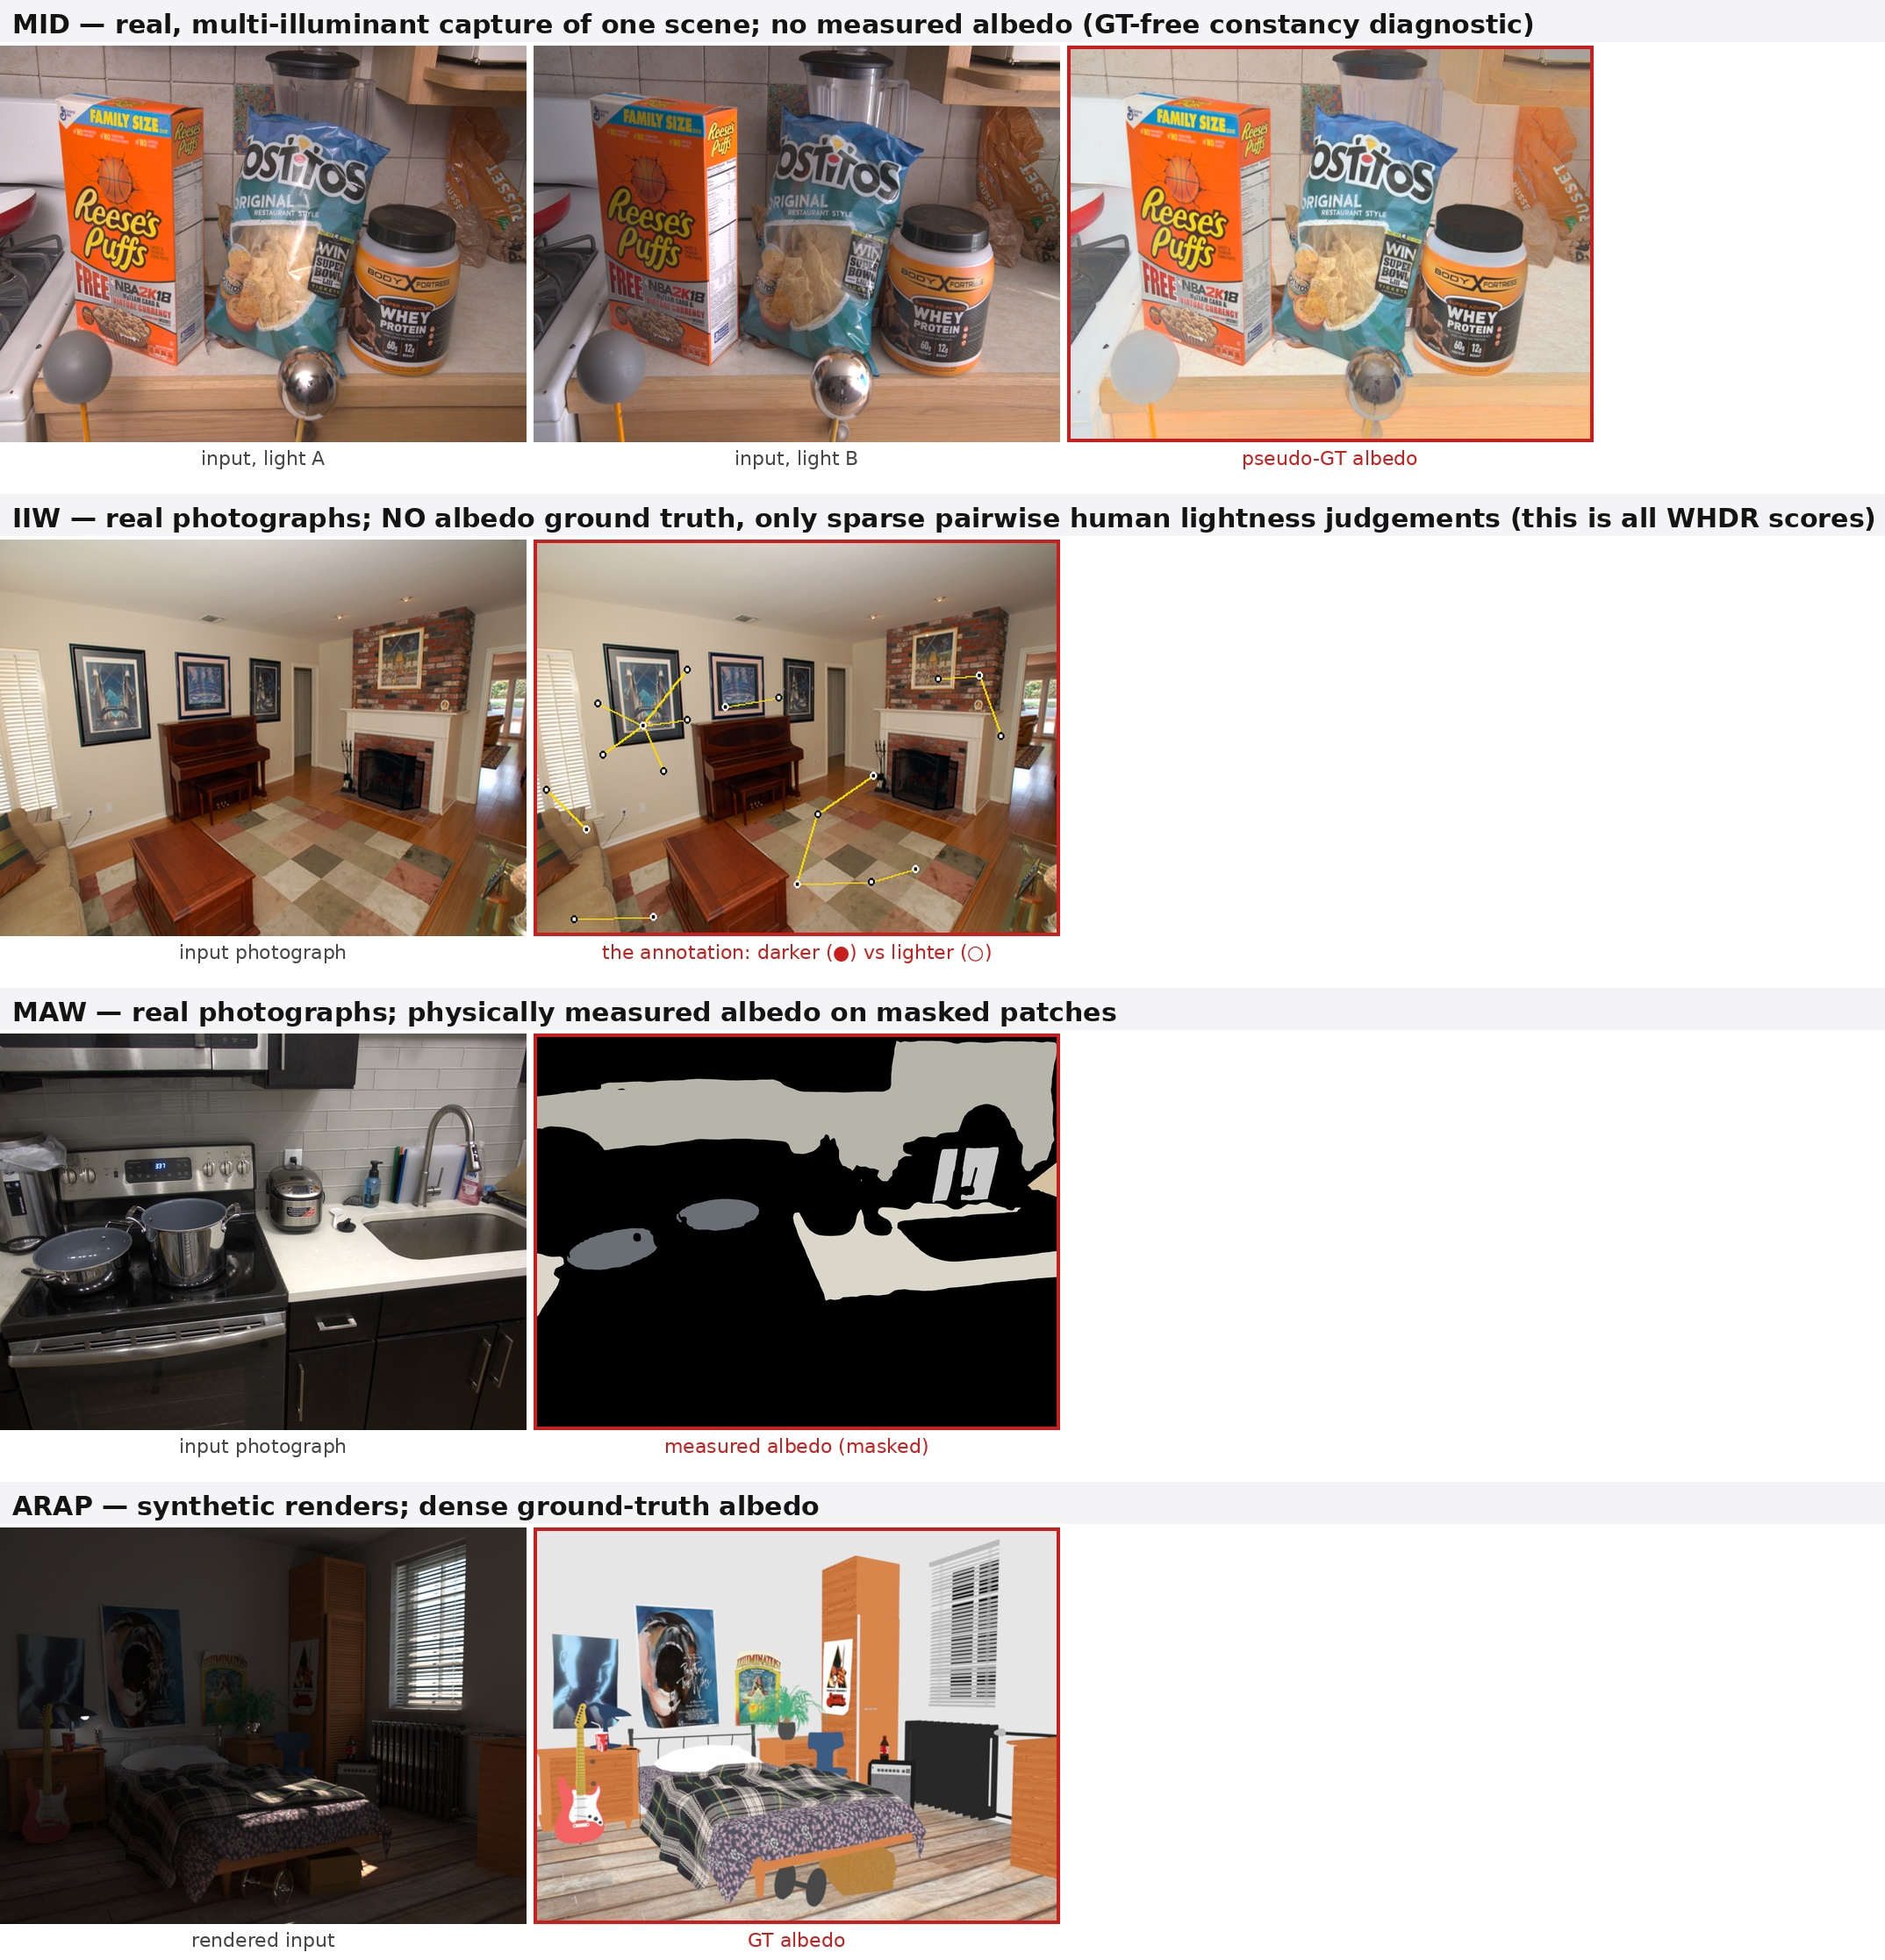
\includegraphics[width=0.92\textwidth]{images/datasets/datasets.jpg}
  \caption[The four evaluation benchmarks and their supervision.]{%
    The four evaluation benchmarks and the ground truth each provides, in the order of \secref{sec:benchmarks}.
    \textbf{MID}: real multi-illuminant captures of one scene, with no measured albedo;
    which is why it supports a ground-truth-free constancy diagnostic and nothing stronger.
    \textbf{IIW}: real photographs with \emph{no} albedo ground truth at all. The second
    panel overlays the annotation that does exist: sparse pairwise human lightness
    judgements, each a pair of points one of which was called darker ($\bullet$) than the
    other ($\circ$). These sparse ordinal comparisons define what WHDR scores;
    they are informative about relative lightness but not RGB colour.
    \textbf{MAW}: real photographs with physically measured albedo on masked patches.
    \textbf{ARAP}: synthetic renders with dense ground-truth albedo.
  }
  \label{fig:datasets}
\end{figure}

\subsection{IIW}

Intrinsic Images in the Wild \mycite{bell14iiw} is the most widely used benchmark
in the IID literature.
It contains 5,230 real indoor and outdoor photographs collected from the internet,
annotated with human pairwise reflectance comparisons.
The evaluation metric is WHDR: the fraction of annotator pairs (weighted by
confidence) with which the model's albedo ordering disagrees.
Lower WHDR is better.
We evaluate on the standard test split of 1,046 images (every fifth image of the
5,230), and report WHDR as the mean over images rather than pooled over
judgements.

\subsection{MID: Multi-Illumination Dataset}
\label{sec:mid_dataset}

MID, the Multi-Illumination Dataset of \mycitetext{midintrinsics}, is the dataset
most directly relevant to this work.
It contains over 1{,}000 real indoor scenes, each photographed 25 times from a
fixed viewpoint with a flash bounced in a different direction for every shot, and
a grey and a chrome probe in every frame.
The flash is white, so between two frames the light changes mainly in
\emph{direction and intensity}. Its colour changes only because the bounced light picks up
the colour of the wall or ceiling it reflects from, and only slightly
(\secref{sec:colour_axis} measures how much).
The key property is that the albedo of each surface does not change across the 25
frames; only the light does. MIDIntrinsics \mycite{careaga23ordinal} adds one dense
pseudo-ground-truth albedo per scene, derived from the white-balanced capture stack and
shared by all 25 frames. This makes it possible to measure how much a model's predicted
albedo of each material changes across frames ($C_{\text{mat}}$ for luminance,
$\text{Cast}_{\text{rel}}$ for hue), and how far it lies from the pseudo-ground truth.
A perfectly illumination-invariant model would have zero variation.
We hold out 30 scenes as a test split and report constancy on those; the training
split, whose scenes never overlap with the test split, is used for the CIAI pairs
(\chapref{ch:implementation}).

\subsection{ARAP}
\label{sec:arap_dataset}

ARAP (``As Real As Possible'') is a synthetic high-dynamic-range dataset of
around 50 rendered indoor and outdoor scenes \mycite{arap}.
A subset of scenes ships with multiple renderings under different lighting
conditions (direction, intensity, and in some scenes light colour). Because ARAP
also provides dense ground-truth albedo, it is the only benchmark here on which
stability across lights and accuracy can be measured on the same pixels
(\secref{sec:arap_results}).

\subsection{MAW: Measured Albedo in the Wild}
\label{sec:maw_dataset}

MAW \mycite{maw} is a benchmark of real indoor images with physically measured albedo.
Each surface is photographed twice, once with a grey card of known reflectance resting on it
and once without. Surface and card receive the same light, so the shading cancels in the
ratio of the two measurements and leaves the surface's albedo in absolute terms. MAW
therefore measures material colour on real photographs, which complements the synthetic
ARAP. It reports a colour error $\Delta E$ and an intensity error (\secref{sec:maw_results}).
We evaluate on 874 images from the MAW test split.
